Fehler werden über Gaussche Fehlerfortpflanzung berechnet.

\subsection{Szintillationsdetektor}
\begin{figure}
\centering
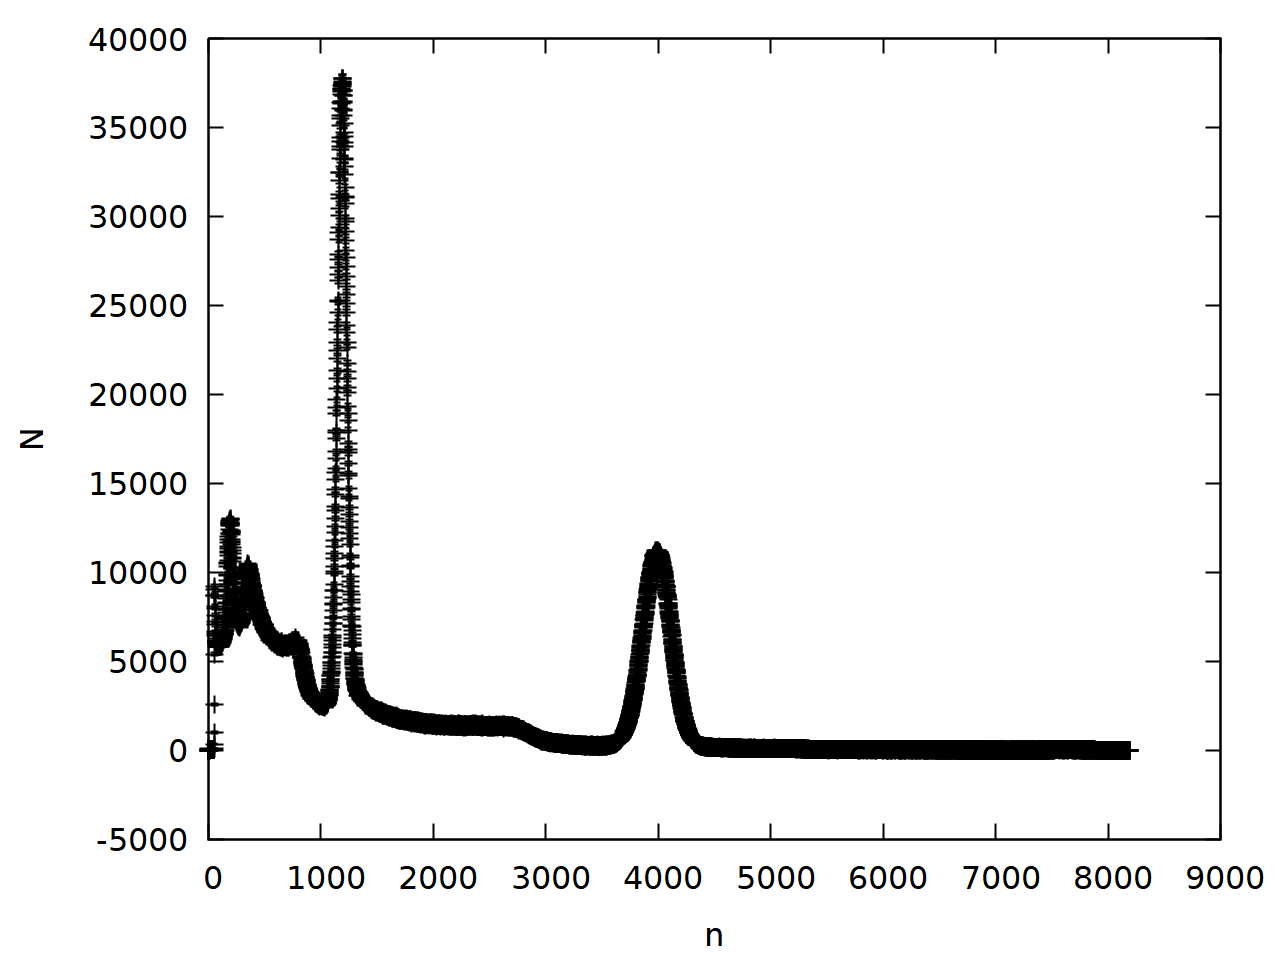
\includegraphics[width=0.7\linewidth]{data/si_cs.png}
\caption{Szintillator Cs korrigiert}
\label{fig:si_cs}
\end{figure}

\begin{figure}
\centering
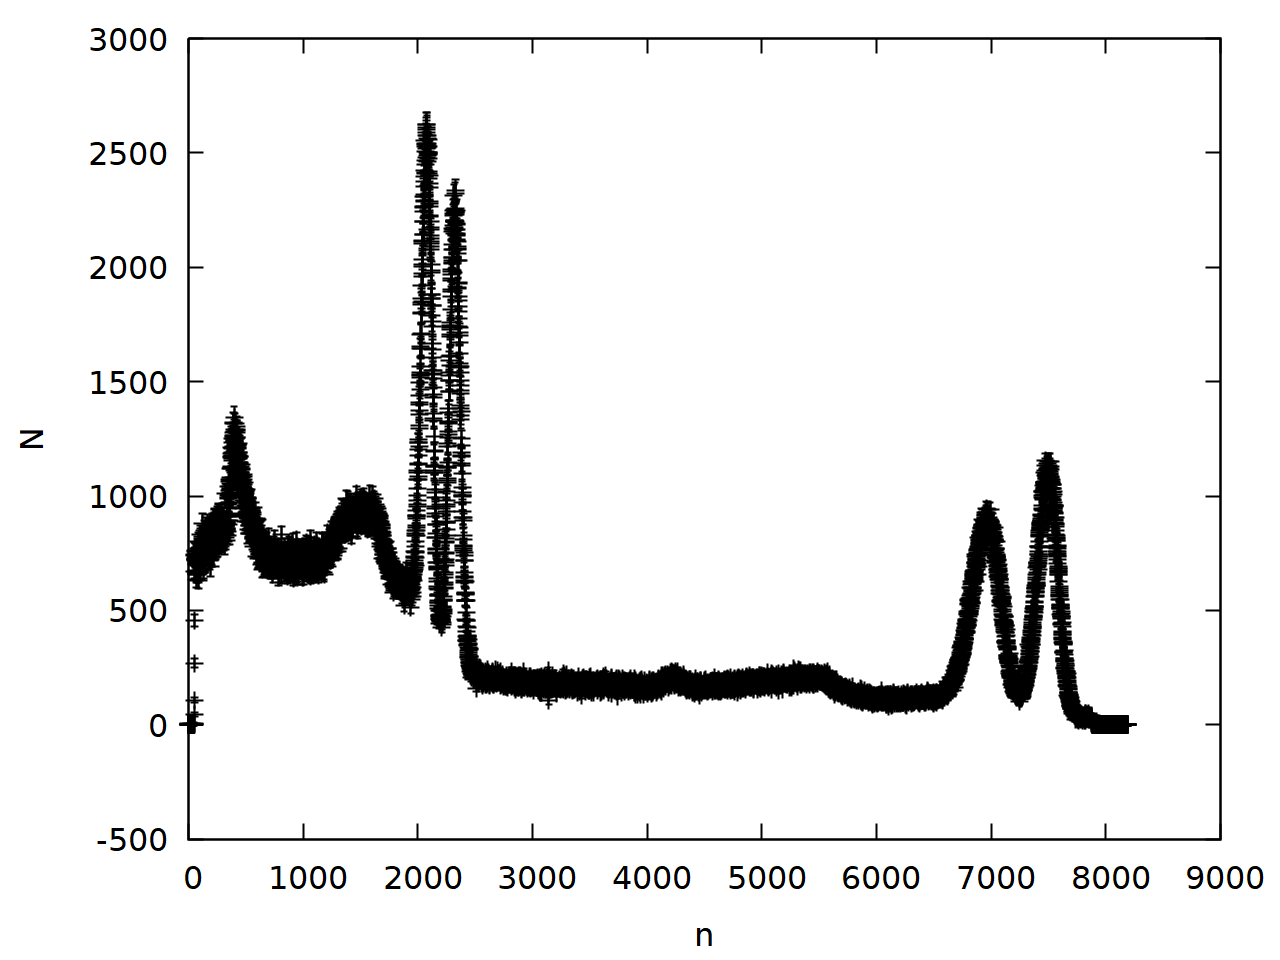
\includegraphics[width=0.7\linewidth]{data/si_co.png}
\caption{Szintillator Co korrigiert}
\label{fig:si_co}
\end{figure}

\begin{figure}
\centering
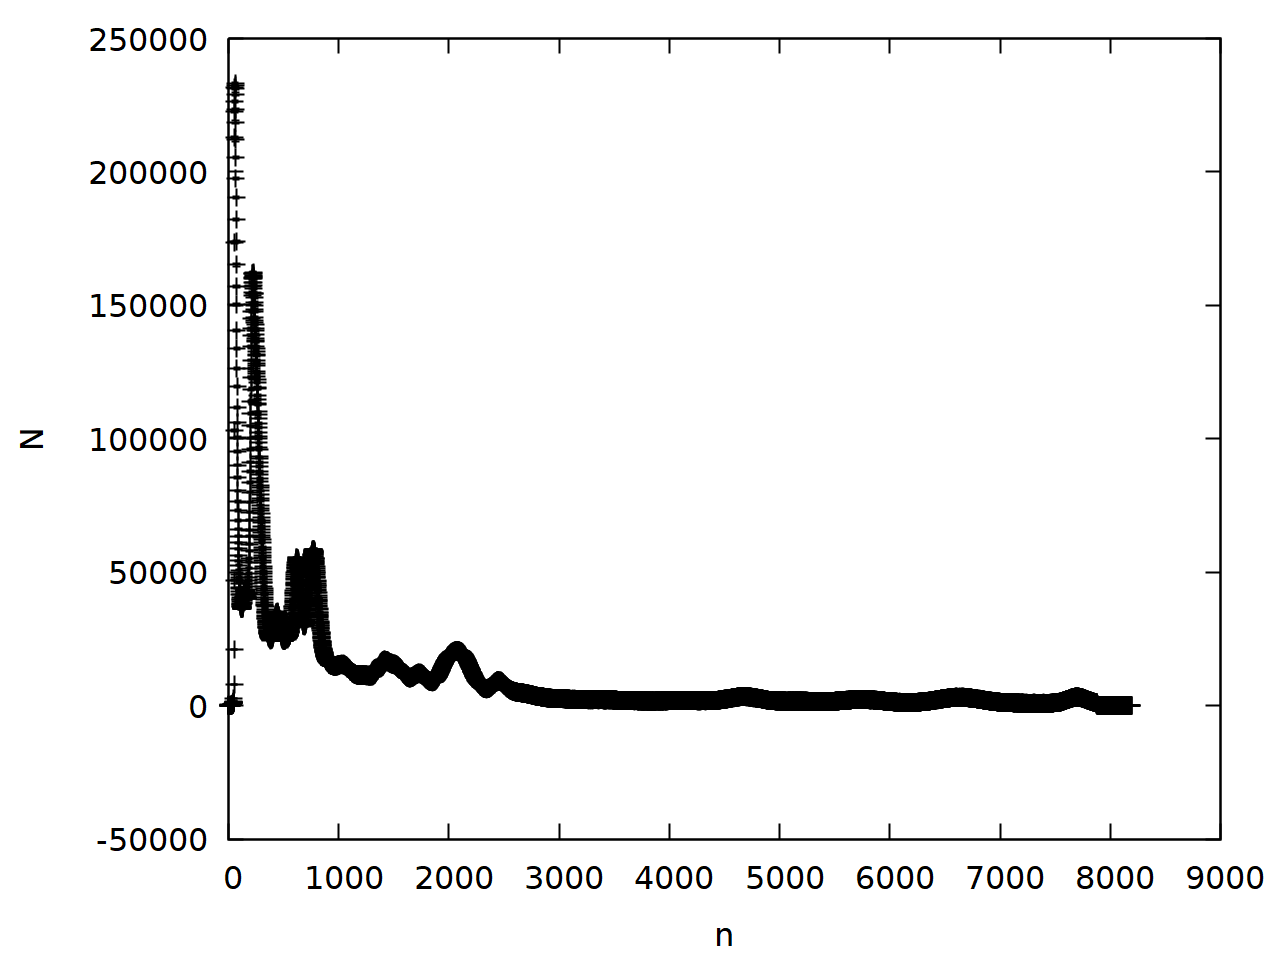
\includegraphics[width=0.7\linewidth]{data/si_eu.png}
\caption{Szintillator Eu korrigiert}
\label{fig:si_eu}
\end{figure}

Die aufgenommenen Spektren im Anhang werden um den Untergrund korrigiert (Werte kleiner 0 werden auf 0 gesetzt) und sind in Abbildung \ref{fig:si_cs} - \ref{fig:si_eu} abgebildet. Als Fehler wird $\sqrt{N}$ angenommen. An die stärksten Linien der 3 Spektren werden nun Gausskurven gefittet\[f(x) = a\exp{\left(-4\ln{2}\frac{(x-b)^2}{\text{FWHM}^2}\right)}\]. Das Ergebnis ist in Tabelle \ref{tab:si} abgebildet (die Halbwertsbreite wurde schon auf keV umgerechnet).

\begin{table}
\caption{Fitergebnisse an den Spektren des Szintillators}
\begin{tabular}{cccccccccc}
\toprule
Peak Nr. & Element & Energie/\si{keV}& $a$ & $\Delta a$ & $b$ & $\Delta b$ & FWHM/\si{keV} & $\Delta \text{FWHM}/\si{keV}$\\
\midrule 
1	&	Cs	&	661,66	&	37781	&	933	&	1193	&	0,9	&	57	&	3\\
2	&	Co	&	1332,5	&	2586	&	90	&	2068	&	1,9	&	82	&	5\\
3	&	Co	&	1173,2	&	2301	&	94	&	2323	&	1,9	&	68	&	4\\
4	&	Eu	&	121,7825	&	160500	&	3181	&	234	&	0,9	&	69	&	4\\
5	&	Eu	&	344,281	&	53500	&	2255	&	610	&	1,8	&	55	&	4\\
6	&	Eu	&	1408,011	&	21300	&	691	&	2055	&	4,9	&	221	&	13\\
\bottomrule
\end{tabular}
\label{tab:si}
\end{table}

Um den Linien die Energie zuzuordnen wurde zuerst der Cäsiumpeak bestimmt. Für Cäsium war uns nur eine Linie (\SI{662}{keV}) vorgegeben. Leider gibt es 2 verschiedene Peaks im Spektrum. Um zu bestimmen, welcher der beiden Peaks der richtige ist, haben wir jeweils den Umrechnungsfaktor Kanal $\leftrightarrow$ Energie abgeschätzt und dann die Energien der restlichen Peaks bestimmt. Bei dem linken Peak gab es eine deutlich bessere Übereinstimmung, so dass wir davon ausgehen, dass dieser Peak der \SI{662}{keV} ist.\\
Um den Umrechnungsfaktor Kanal $\leftrightarrow$ Energie zu bestimmen, tragen wir die Kanalnummer über der Energie der Peaks auf und führen einen linearen Fit \[f(x) = C\ind{Si}\cdot x\] durch (siehe Abbildung \ref{fig:si_gauge}). Als Fehler der Kanalnummer nehmen wir die Standartweichung der Gausskurve an. Der Fit ergibt: $C\ind{Si} = \si{(1,77\pm 0,09)\,Kanal/keV}$

\begin{figure}
\centering
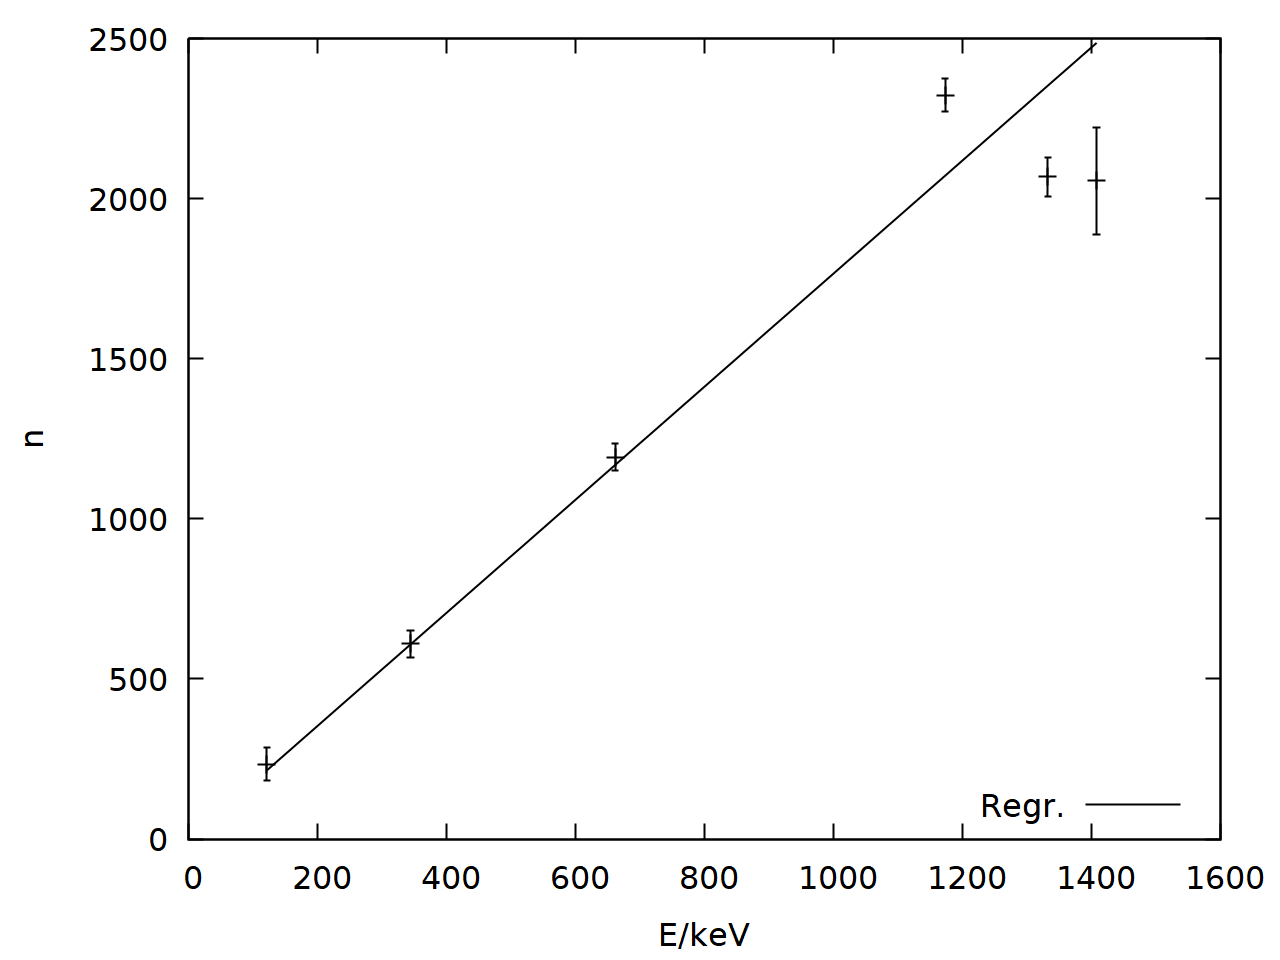
\includegraphics[width=0.7\linewidth]{data/si_gauge.png}
\caption{Szintillator Kalibrierung}
\label{fig:si_gauge}
\end{figure}

\subsubsection*{Peak-to-Total}
Die gesamte Anzahl der untergrundkorrigierten Ereignisse beträgt für Cäsium: $N\ind{total}\upd{Cs} = 17152004 \pm 4141$ und für Cobalt: $N\ind{total}\upd{Co} = 3482320\pm 1866$ (Als Fehler wurde wieder $\sqrt{N}$ angenommen). 
Um die Anzahl der Ereignisse in den Peaks unabhängig vom Kontinuum abzuschätzen, berechnen wir die Fläche unter der jeweiligen Gausskurve \[N\ind{Peak} = a\cdot\sqrt{2\pi}\cdot \sigma\], wobei $\sigma$ die Standartabweichung der Gausskurve ist.
Damit ergibt sich für den Cs-Peak: $\text{PtT}\upd{Cs} = \cfrac{N\ind{Peak}\upd{Cs}}{N\ind{total}\upd{Cs}} = 0,237\pm 0,007$ und die beiden Cobaltpeaks (diese werden nach Praktikumsanleitung zusammenaddiert): $\text{PtT}\upd{Co} = 0,198\pm 0,007$.

\subsection{Halbleiter-Detektor}
\begin{figure}
\centering
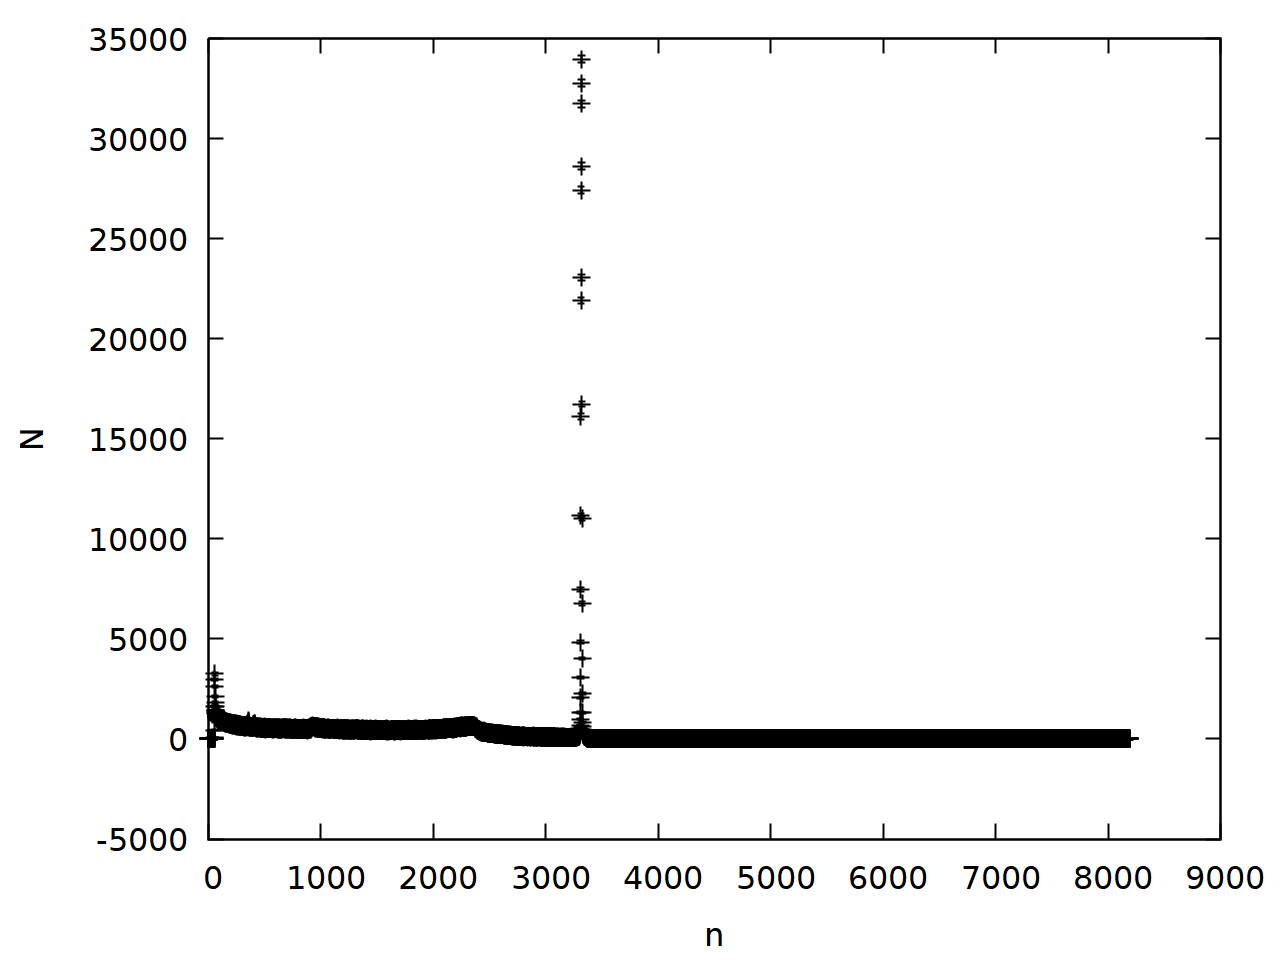
\includegraphics[width=0.7\linewidth]{data/ge_cs.png}
\caption{Halbleiter Cs korrigiert}
\label{fig:ge_cs}
\end{figure}

\begin{figure}
\centering
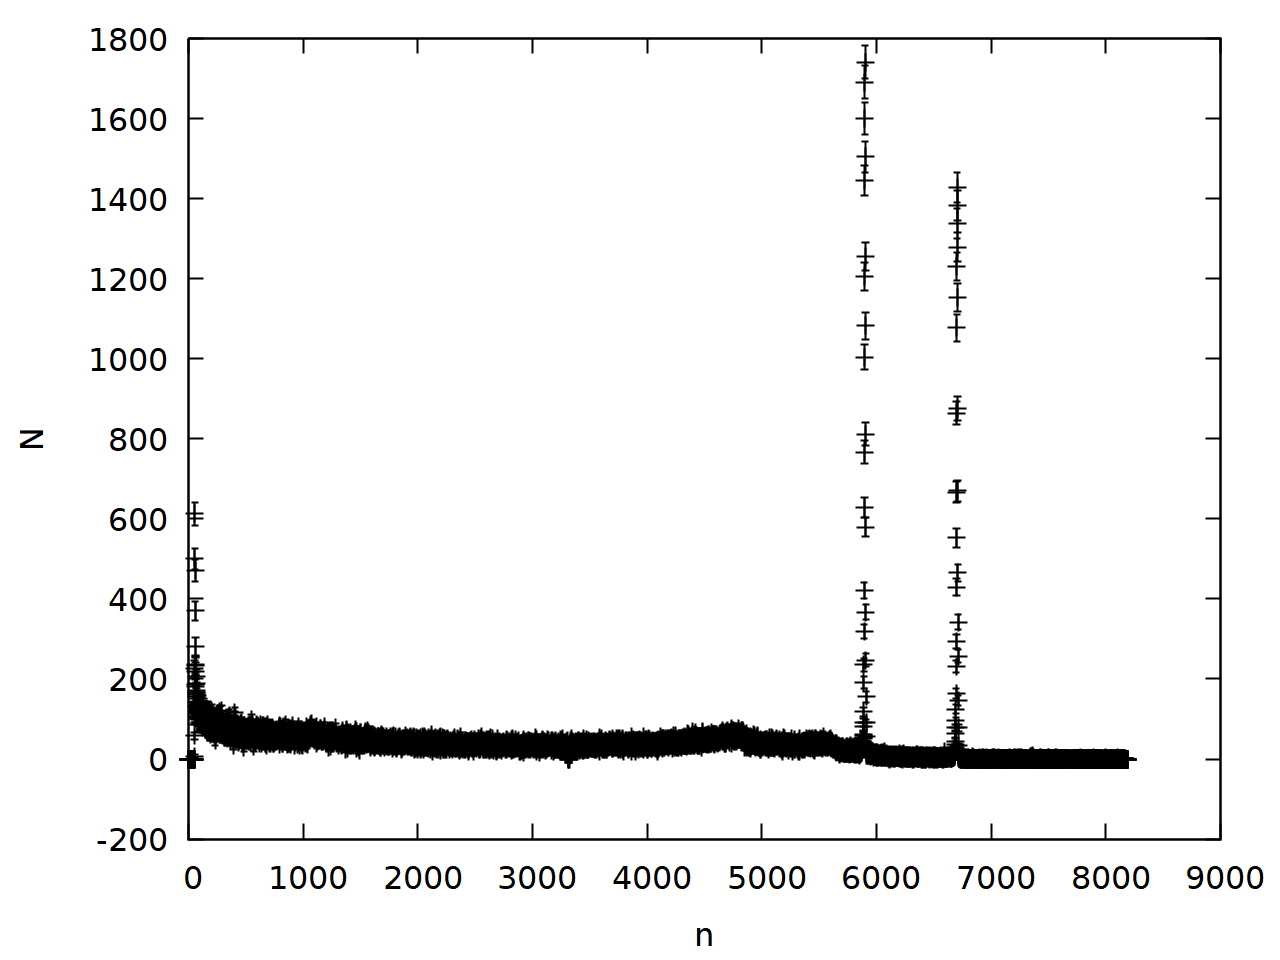
\includegraphics[width=0.7\linewidth]{data/ge_co.png}
\caption{Halbleiter Co korrigiert}
\label{fig:ge_co}
\end{figure}

\begin{figure}
\centering
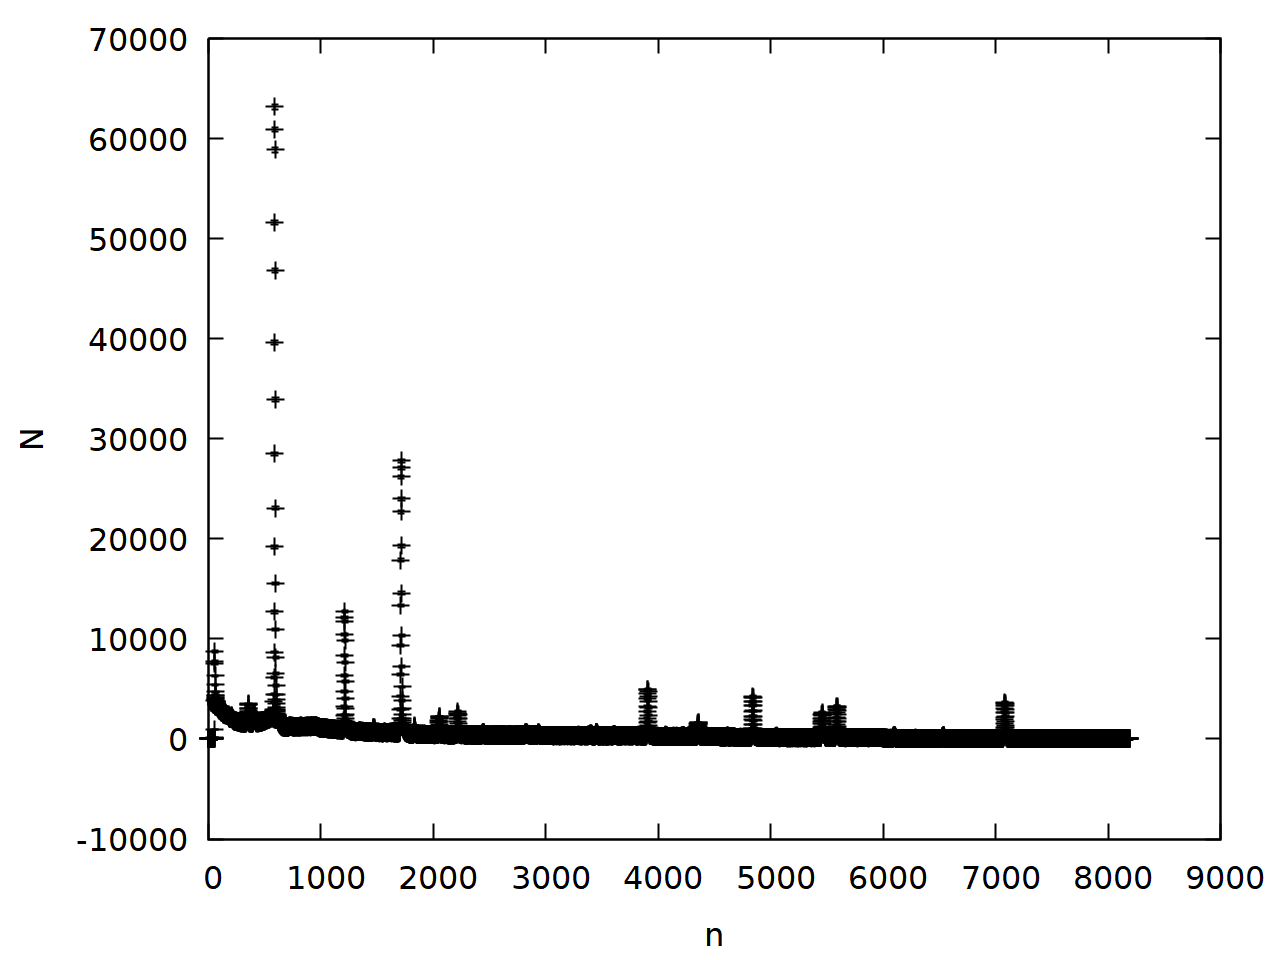
\includegraphics[width=0.7\linewidth]{data/ge_eu.png}
\caption{Halbleiter Eu korrigiert}
\label{fig:ge_eu}
\end{figure}

Die Auswertung des Halbleiterdetektors geschieht analog zur Auswertung des Szintillators. In den Abbildungen \ref{fig:ge_cs} - \ref{fig:ge_eu} sind die gemessenen Spektren der Proben abgebildet. Wieder werden Gausskurven an die Peaks gefittet (siehe Tabelle \ref{tab:ge}). Die Zuordnung des Cäsiumpeaks ist bei diesem Detektor einfacher, weil sich nur ein Peak im Bereich befindet. Vergleicht die Form des Spektrums in der Umgebung des Peaks, so kann man erkennen, dass es sich um den gleichen Peak wie beim Szintillator handelt.\\

\begin{table}
\caption{Fitergebnisse an den Spektren des Halbleiterdetektor}
\begin{tabular}{cccccccccc}
\toprule
Peak Nr. & Element & Energie/\si{keV}& $a$ & $\Delta a$ & $b$ & $\Delta b$ & FWHM/\si{keV} & $\Delta \text{FWHM}/\si{keV}$\\
\midrule 
1	&	Cs	&	661,66	&	32170	&	796	&	3316,9	&	0,1	&	1,68	&	0,03\\
2	&	Co	&	1173,2	&	1596	&	77	&	5899,8	&	0,2	&	2,06	&	0,06\\
3	&	Co	&	1332,5	&	1427	&	63	&	6704,0	&	0,2	&	1,79	&	0,06\\
4	&	Eu	&	121,78	&	56415	&	11932	&	591,8	&	0,6	&	1,56	&	0,23\\
5	&	Eu	&	244,6989	&	10944	&	5376	&	1212,9	&	1,5	&	1,61	&	0,59\\
6	&	Eu	&	344,281	&	25549	&	7567	&	1715,2	&	0,9	&	1,73	&	0,35\\
7	&	Eu	&	778,903	&	4691	&	3072	&	3908,0	&	2,4	&	1,99	&	0,97\\
8	&	Eu	&	964,131	&	4056	&	2667	&	4843,0	&	2,6	&	2,19	&	1,05\\
9	&	Eu	&	1085,914	&	2527	&	2133	&	5458,0	&	3,5	&	2,19	&	1,42\\
10	&	Eu	&	1112,116	&	3121	&	2389	&	5590,0	&	3,2	&	2,19	&	1,26\\
11	&	Eu	&	1408,011	&	3655	&	2361	&	7084,0	&	2,8	&	2,39	&	1,08\\
\bottomrule
\end{tabular}
\label{tab:ge}
\end{table}

Nachdem man den Peaks die Energien zugeordnet hat, wird wieder zur Kalibration der Kanal über der Energie aufgetragen (siehe Abbildung \ref{fig:ge_gauge}). Ein linearer Fit ergibt: $C\ind{Ge} = \si{(5,025\pm 0,004)\,Kanal/keV}$

\begin{figure}
\centering
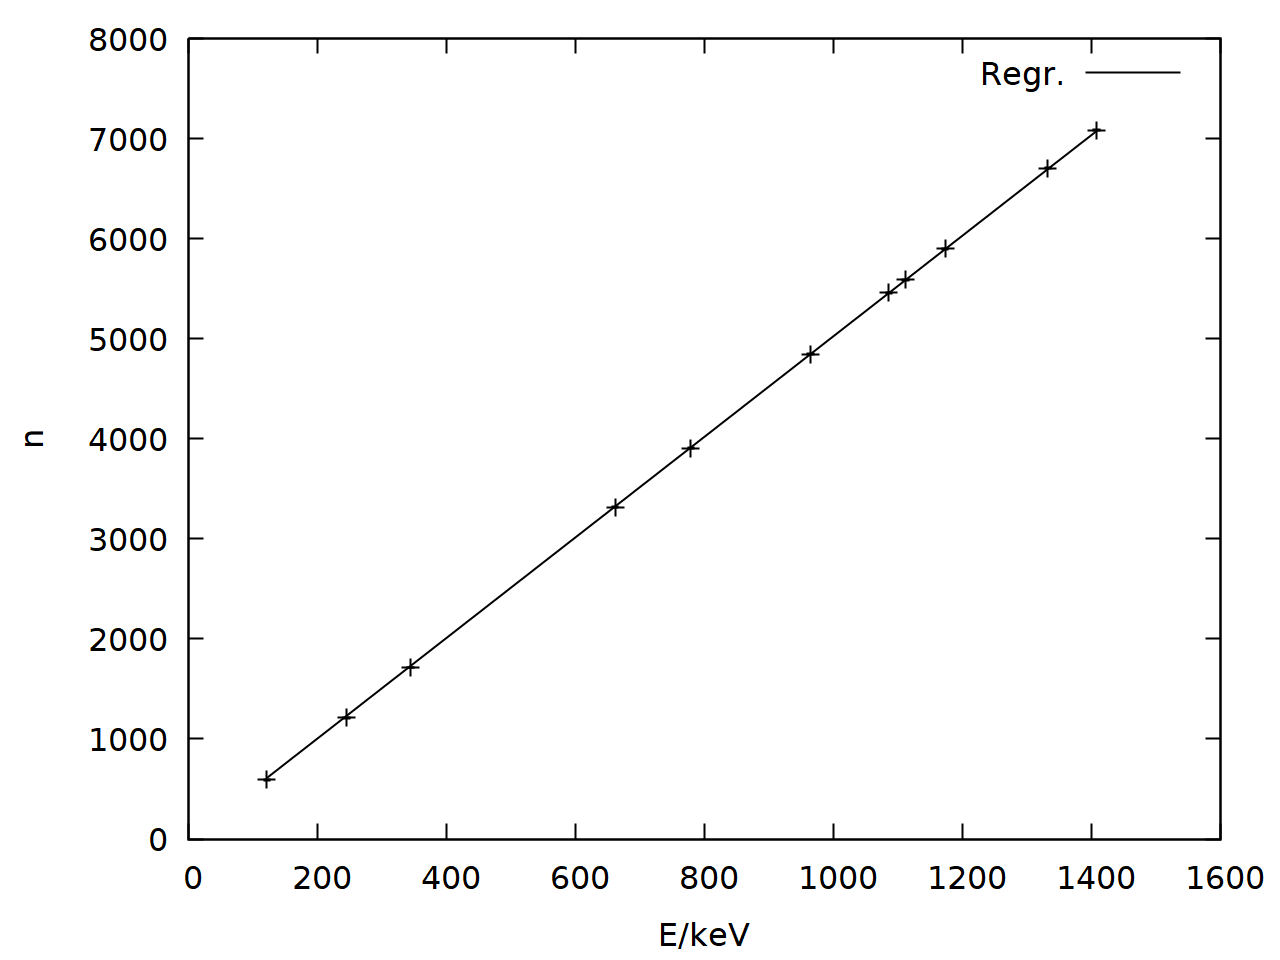
\includegraphics[width=0.7\linewidth]{data/ge_gauge.png}
\caption{Halbleiter Kalibrierung}
\label{fig:ge_gauge}
\end{figure}

\subsubsection*{Intrinsische Halbwertsbreite}
Die Halbwertsbreite eines Peaks ist laut Praktikumsheft \cite{praktikumsheft} gegeben durch:
\begin{align*}
\Delta E^2 = c \cdot E + \Delta E\ind{e}^2
\end{align*}
Dieser Zusammenhang wird überprüft, indem die Quadrate der Halbwertsbreiten der Eu-Linien über der Energie aufgetragen werden (siehe Abbildung \ref{fig:ge_intrinsic}). Man kann erkennen, dass die Werte gut auf einer Geraden liegen. Ein linearer Fit ergibt: $c = \si{(2,5 \pm 0,1)\cdot 10^{-3}\,keV}$ und $\Delta E\ind{e}^2 = \si{(2,13 \pm 0,03)\,keV^2}$. Damit folgt, dass der elektronische Anteil der Halbwertsbreite $\Delta E\ind{e} = \si{(1,46 \pm 0,01)\,keV}$ ist.

\begin{figure}
\centering
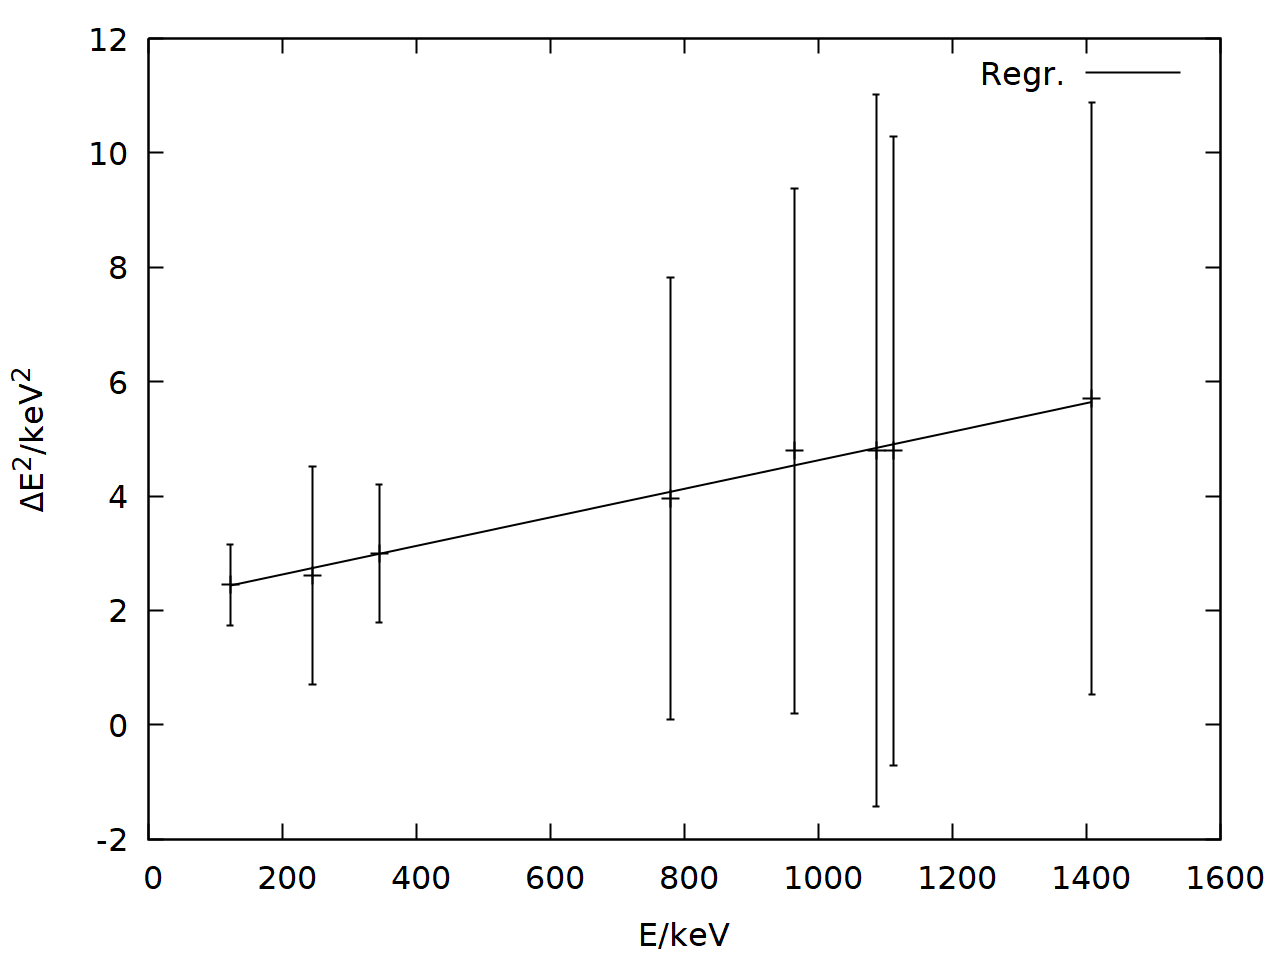
\includegraphics[width=0.7\linewidth]{data/ge_intrinsic.png}
\caption{Halbleiter Intrinsische Halbwertsbreite}
\label{fig:ge_intrinsic}
\end{figure}


\subsubsection*{Peak-to-Total}
Die gesamte Anzahl der untergrundkorrigierten Ereignisse beträgt für Cäsium: $N\ind{total}\upd{Cs} = 1762931 \pm 1328$ und für Cobalt: $N\ind{total}\upd{Co} = 304614\pm 552$.\\
Damit ergibt sich für den Cs-Peak: $\text{PtT}\upd{Cs} = 0.163\pm 0,005$ und die beiden Cobaltpeaks: $\text{PtT}\upd{Co} = 0.103\pm 0,004$. Das PtT-Verhältnis ist also für den Halbleiter kleiner als für den Szintillator.

\subsubsection*{Relative Effizienz als Funktion der Gammaenergie}
Um die relative Effizienz des Detektors zu bestimmen, wird das Verhältnis aus der Amplitude der Gausskurve an einem Eu-Peak mit der Amplitude des \SI{1408}{keV}-Peaks gebildet. Dieses wird mit 1000 multipliziert und dann durch den angegebenen Wert im Praktikumsheft \cite{praktikumsheft}(Tabelle P521.6.1.) geteilt. Die Werte werden über der Energie aufgetragen (siehe Abbildung \ref{fig:ge_relint}).

\begin{figure}
\centering
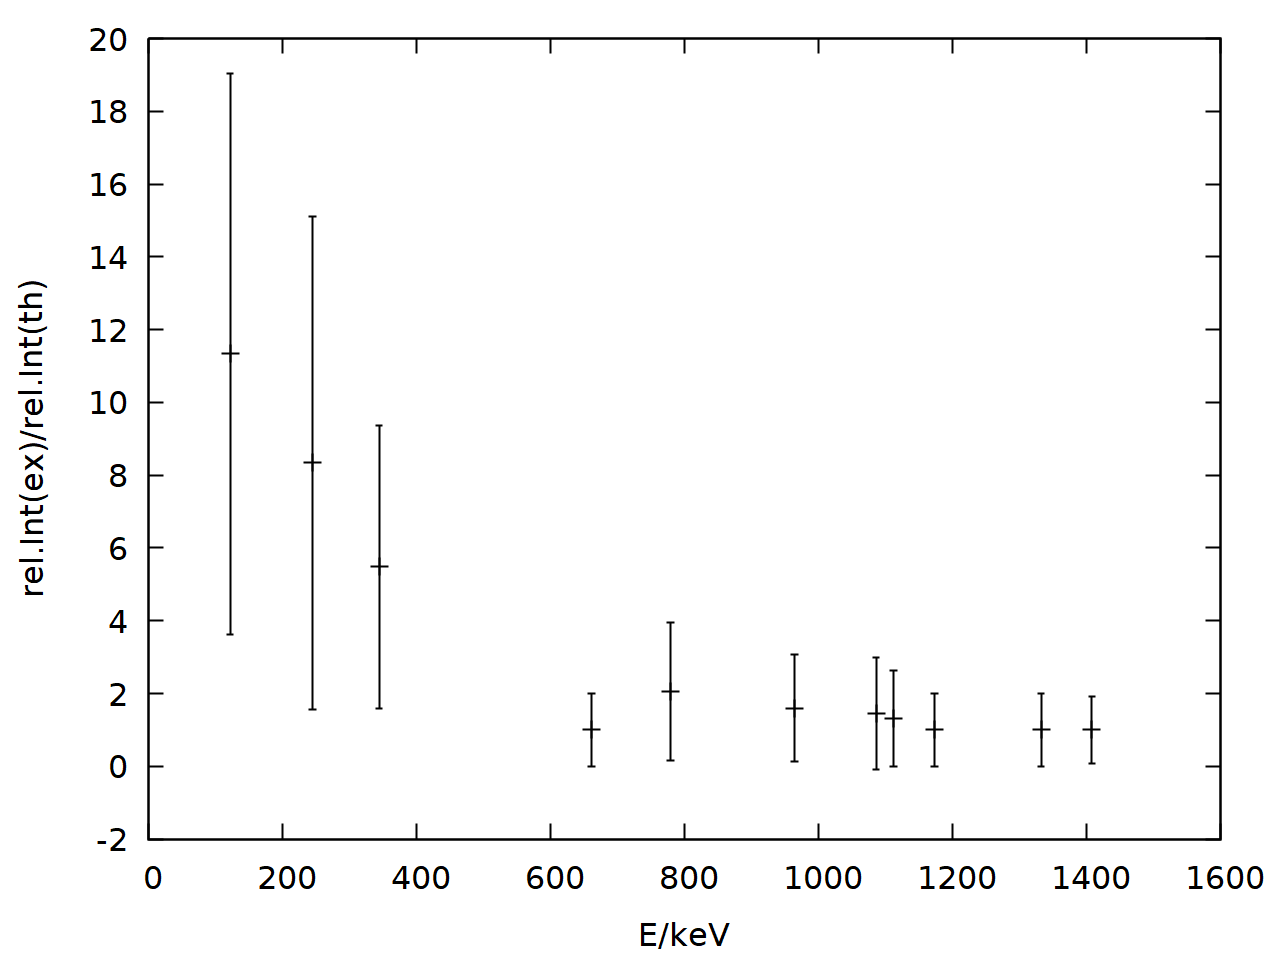
\includegraphics[width=0.7\linewidth]{data/ge_relint.png}
\caption{Halbleiter relative Effizienz}
\label{fig:ge_relint}
\end{figure}

Wäre der Detektor in allen Energiebereichen gleich effizient, so lägen alle Werte auf einer Höhe. Die Effizienz fällt aber bei kleinen Energien ab und ist danach in etwa konstant. Das bedeutet, dass der Detektor effizienter bei kleinen Energien ist, während er bei großen Energien gleichmäßig effizient ist.

\subsection{Bodenprobe}
Von Langzeitmessung der Bodenprobe (siehe Anhang) wird der Untergrund abgezogen(Abbildung \ref{fig:erde}). Werte kleiner als 0 wurden dabei nicht auf 0 gesetzt, um erkennen zu können, ob die Bodenprobe abschirmend wirkt. Als Fehler wird $\sqrt{N}$ oder $1$ angenommen, wenn die Zahl kleiner gleich 0 ist.

\begin{figure}
\centering
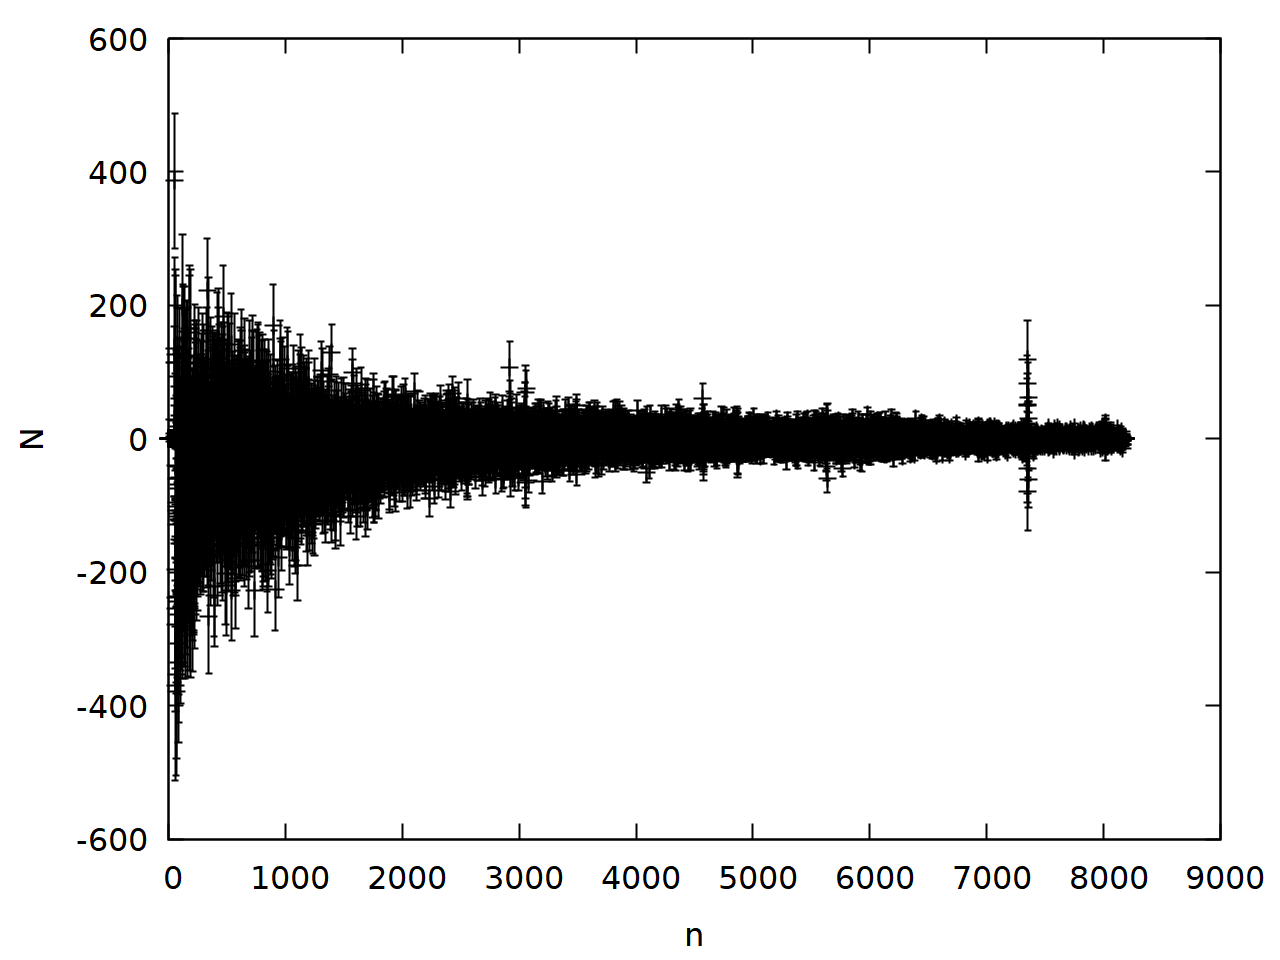
\includegraphics[width=0.7\linewidth]{data/erde.png}
\caption{Bodenprobe Untergrundkorrigiert}
\label{fig:erde}
\end{figure}

Man kann erkennen, dass bei kleinen Energien die negativen Werte betragsmäßig größer sind. Daraus kann man schließen, dass ohne Bodenprobe weniger Untergrundteilchen den Detektor erreicht haben, also die Bodenprobe den Untergrund abgeschirmt hat. Weiterhin kann man in dem Spektrum nur eine Linie erkennen (ansonsten gibt es nur einzelne Punkte, die vom Kontinuum abweichen; diese können prinzipiell rein statistischer Natur sein). Da diese Linie allerdings auch negative Werte aufweist, die betragsmäßig genauso groß sind, gehen wir davon aus, dass diese Linie die gleiche Linie wie im Untergrundspektrum ist. Das kann man bestätigen, in dem man die Rohdaten betrachtet. In beiden Spektren ist der Peak etwa gleich hoch und somit keine Linie der Probe, sondern des Untergrundes. Somit enthält unsere Bodenprobe keine sichtbaren Gammalinien.\\

Aufgrund dessen wurde das Spektrum des Untergrundes untersucht. Dazu werden wie zuvor an die deutlichsten Peaks und an den Cäsiumpeak Gausskurven gefittet. Die Kanalnummber $b$ wird über $C\ind{Ge}$ in eine Energie umgerechnet. Diese werden mithilfe von \cite{lara} Nukliden zugeordnet. Es konnten mehrere Linien der Uran-Actinium-Reihe gefunden werden ($^{227}$Ac, $^{223}$Ra, $^{227}$Th) und eine Linie der Uran-Radium-Reihe ($^{226}$Ra). Die $^{40}$K-Linie ist nicht Teil einer Zerfallsreihe sondern ist Teil des natürlich in der Umwelt vorkommenden Kaliums. Deswegen ist es auch Teil des Untergrundes. Das Nuklid $^{137}$Cs stammt von der Reaktorkatastrophe in Tschernobyl. Die Höhe des Peaks ist aber mit $(1,6 \pm 0,3) \cdot 10^3$ Ereignissen vergleichsweise klein (z.B. Kalium: $(19 \pm 3)\cdot 10^3$). Somit ist die Belastung mit Cäsium vergleichsweise gering.

\begin{table}
\caption{Fitergebnisse an das Untergrundspektrum}
\begin{tabular}{ccccccccccc}
\toprule
Peak Nr. & $a$ & $\Delta a$ & $b$ & $\Delta b$ & FWHM/\si{keV} & $\Delta \text{FWHM}/\si{keV}$& E/\si{keV}& $\Delta\text{E}/\si{keV}$ & Nuklid & Zerfallsreihe\\
\midrule 
1	&	4564	&	4155	&	356,7	&	1,7	&	1,9	&	2,0	&	71,0	&	0,3	&	$^{227}$Ac, $^{223}$Ra\\
2	&	8227	&	3456	&	1184,0	&	1,0	&	2,4	&	1,1	&	235,6	&	0,5	&	$^{227}$Ac\\
3	&	6142	&	2661	&	1755,4	&	1,2	&	2,8	&	1,3	&	349,3	&	0,6	&	$^{226}$Ra \\
4	&	4555	&	2048	&	2922,5	&	1,5	&	3,5	&	1,6	&	581,6	&	0,8	&	$^{227}$Ac \\
5	&	6258	&	2251	&	3053,9	&	1,2	&	3,4	&	1,2	&	607,7	&	0,8	&	$^{227}$Ac, $^{227}$Th\\
6	&	1677	&	287	&	3317,7	&	0,8	&	4,5	&	0,8	&	660,2	&	0,9	&	$^{137}$Cs & -\\
7	&	19092	&	3230	&	7351,5	&	0,8	&	5,6	&	0,7	&	1463,0	&	1,6	&	$^{40}$K & -\\
\bottomrule
\end{tabular}
\label{tab:ge}
\end{table}